\documentclass[answers]{exam}
\usepackage{../../mypackages}
\usepackage{../../macros}


\SolutionEmphasis{\color{blue}}
\renewcommand{\solutiontitle}{\noindent}


\title{DST N°3 - Géométrie dans l'espace et Sections}
\author{N. Bancel}
\date{22 Janvier 2024}

\begin{document}

\textbf{Collège Lycée Suger}
\hfill
\textbf{Mathématiques} \\

\textbf{Année 2024-2025 - 2ème trimestre}
\hfill
\textbf{1ères STD2A} \par

{\let\newpage\relax\maketitle}

\begin{center}
\textbf{\textcolor{red}{Durée : 2 heures. La calculatrice n'est pas autorisée}} \\
\textbf{\textcolor{red}{Une réponse donnée sans justification sera considérée comme fausse.}} \\
Cette interrogation contient \numquestions\ questions, sur \numpages\ pages et est notée sur 20 points. 

\end{center}

\section*{Exercice 1 : Figures régulières et tranformations (6 points)}


\vspace{1em}

\begin{questions}
  \question[2] Construire la translation de vecteur $\overrightarrow{u}$ de la figure ci-dessous. Justifier.
  \begin{figure}[H]
    \centering
    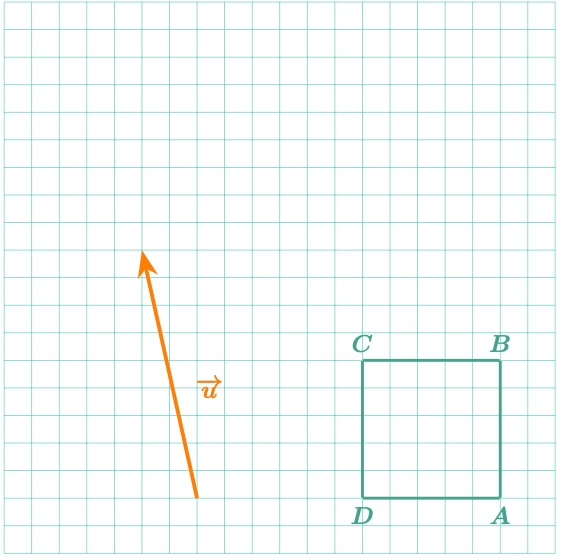
\includegraphics[width=0.4\linewidth]{img/dst_03_01.jpg}
  \end{figure}

  \question[2] Quelle est la nature de la transformation qui transforme la figure verte en la figure rouge ? Justifier que la réponse est bien correcte pour chaque point de la figure. 

  \begin{figure}[H]
    \centering
    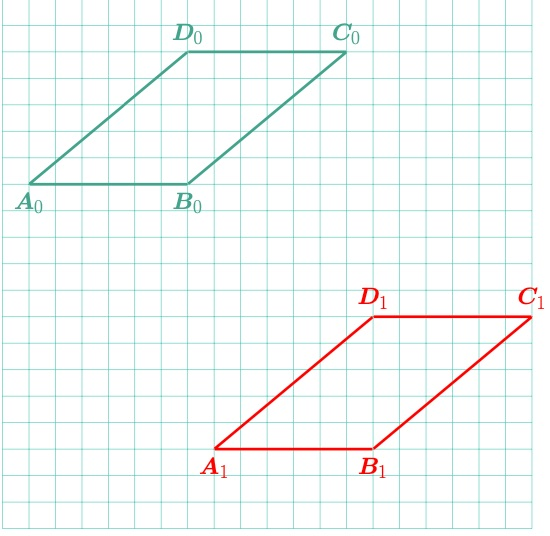
\includegraphics[width=0.4\linewidth]{img/dst_03_02.jpg}
  \end{figure}

  \question[2] Construire la rotation de centre E et d’angle $45°$ (sens horaire) pour la figure ci-dessous. Justifier pour chaque point de la figure.

  \begin{figure}[H]
    \centering
    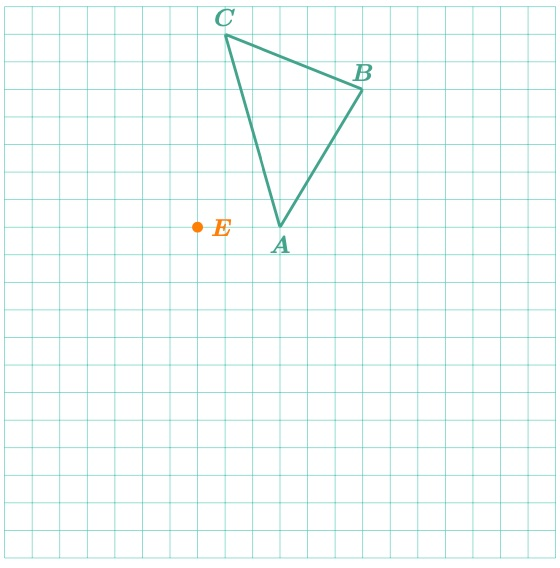
\includegraphics[width=0.4\linewidth]{img/dst_03_03.jpg}
  \end{figure}

\end{questions} 


\section*{Exercice 2 : Section - Cours (4 points)}

\begin{questions} 
\question[0.5] Combien de points faut-il pour déterminer / délimiter un plan ? Combien faut-il de droites ?
\begin{solution}
  Il faut au moins \textbf{trois points non alignés} pour déterminer un plan.  
  On peut aussi définir un plan avec \textbf{deux droites sécantes} ou \textbf{deux droites parallèles}.
  \end{solution}
\question[0.5] Qu'est ce qui permet de dire que 2 plans sont parallèles ?
\begin{solution}
  Deux plans sont parallèles s'ils n'ont \textbf{aucun point d'intersection}, c'est-à-dire qu'ils ne se coupent jamais.  
  Une autre caractérisation est que s'ils contiennent \textbf{deux droites parallèles entre elles}, alors ils sont parallèles.
  \end{solution}
\question[0.5] Si deux plans ne sont pas parallèles, quelle est la forme de leur intersection ? 
\begin{solution}
  Si deux plans ne sont pas parallèles, ils sont \textbf{sécants} et leur intersection est une \textbf{droite}.
  \end{solution}
\question[1.5] Soit deux plans parallèles $P$ et $P'$. Soit un plan $Q$ qui coupe à la fois le plan $P$ et le plan $P'$ en respectivement deux droites $\Delta$ et $\Delta'$. Que peut-on dire des droites $\Delta$ et $\Delta'$ ? Une justification accompagnée d'un dessin rapporte plus de points.
\begin{solution}
  Les droites $\Delta$ et $\Delta'$ sont \textbf{parallèles}.  
  En effet, puisque le plan $Q$ coupe les deux plans parallèles $P$ et $P'$, les droites $\Delta$ et $\Delta'$ sont les intersections respectives de $Q$ avec $P$ et $P'$. Or, lorsqu'un plan coupe deux plans parallèles, les droites d'intersection sont elles-mêmes parallèles.  
  
  Un dessin illustrant cette propriété peut être ajouté pour clarifier la réponse.
  \end{solution}  
\question[1] Enoncer le théorème du toit. Un dessin peut être fait pour illustrer la réponse.
\begin{solution}
  Le \textbf{théorème du toit} affirme que :  
  
  Si deux droites \textbf{parallèles} sont contenues respectivement dans deux plans \textbf{distincts} et \textbf{sécants}, alors l'intersection de ces deux plans est \textbf{parallèle} aux deux droites données.
  
  Un dessin illustrant ce théorème avec deux plans sécants et deux droites parallèles dans ces plans peut être ajouté.
  \end{solution}
\end{questions} 

\section*{Exercice 3 : Section - Exercice (3 points)}

\begin{questions} 
  \question[3] Tracer la section du cube $ABCDEFGH$ par le plan $(IJK)$, en décrivant chacune des étapes de construction de celle-ci. Une justification est obligatoire.
\end{questions} 

\begin{figure}[H]
  \centering
  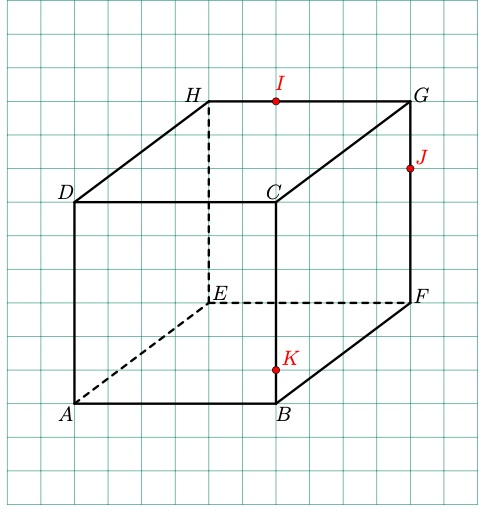
\includegraphics[width=0.8\linewidth]{img/dst_03_04.jpg}
\end{figure}

\section*{Exercice 4 : Géométrie dans l'espace - (7 points)}


\textbf{Extrait du BAC 2017 STD2A Nouvelle Calédonie} \par
\vspace{1em}
Dans les jeux de rôles, on utilise différents types de dés en plus du classique dé à six faces afin
d'obtenir des résultats différents. Les polyèdres réguliers, connus aussi sous le nom de "solides de
Platon", permettent d'obtenir des dés équiprobables, chaque face ayant la même probabilité de
sortir à chaque tirage. Par exemple, un dé à huit faces a la forme d'un octaèdre régulier.

\subsection*{Étude de l'octaèdre régulier}

Un octaèdre régulier peut-être obtenu à partir d'un cube en prenant pour sommets de l'octaèdre les centres des faces du cube.
On a représenté ci-dessous, en perspective parallèle, un octaèdre régulier ABCDEF inscrit dans un cube dont l'arête mesure 2 cm.
Le point O est le point d'intersection des diagonales du quadrilatère ABCD

\begin{figure}[H]
  \centering
  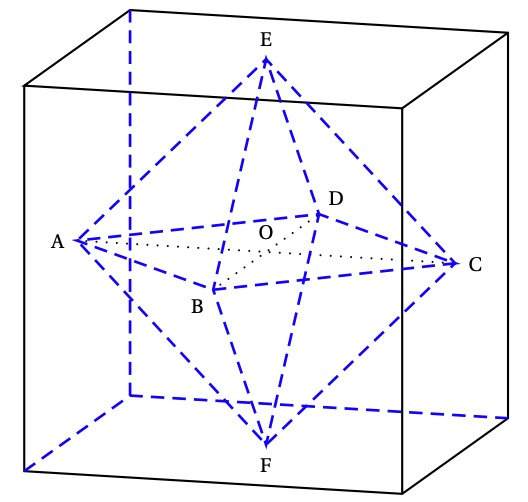
\includegraphics[width=0.4\linewidth]{img/dst_02_01.jpg}
  \caption{\label{} Octaèdre}
\end{figure}

On admet que $\left(O\mathpunct{} ; \ \overrightarrow{OA}\mathpunct{}, \ \overrightarrow{OB}\mathpunct{}, \ \overrightarrow{OE}\right)$ est un repère orthonormal de l'espace.
\begin{questions}
  \question[2] Donner les coordonnées des sommets de l'octaèdre régulier ABCDEF dans le repère orthonormal de l'espace $\left(O\mathpunct{} ; \ \overrightarrow{OA}\mathpunct{}, \ \overrightarrow{OB}\mathpunct{}, \ \overrightarrow{OE}\right)$
  \begin{solution}

  Le repère étant orthonormal, son unité de "mesure" est 1. $\left(O\mathpunct{} ; \ \overrightarrow{OA}\mathpunct{}, \ \overrightarrow{OB}\mathpunct{}, \ \overrightarrow{OE}\right)$ nous permet de dire que 
  \begin{itemize}[noitemsep]
    \item $OA = 1$ La longueur OA vaut 1. Il en est de même pour $OB$ et $OE$. $OA = OB = OE = 1$
    \item En terme de directions : la direction $\overrightarrow{OA}$ indique le sens des "x postifs". La direction $\overrightarrow{OB}$ indique le sens des "y positifs". La direction $\overrightarrow{OE}$ indique le sens des "z positifs".
  \end{itemize}

  Il faut toujours commencer par donner les coordonées des points qui définissent le repère orthonormé. C'est plus simple. Ainsi, on peut donner les coordonées suivantes : 
  \begin{itemize}[noitemsep]
    \item $A(1,0,0)$
    \item $B(0,1,0)$
    \item $E(0,0,1)$
    \item C est au même niveau que A sur les Y et les Z, mais il est à l'opposé de A sur les X : $C(-1,0,0)$
    \item D est au même niveau que B sur les X et les Z, mais il est à l'opposé de B sur les Y : $D(0,-1,0)$
    \item F est au même niveau que E sur les X et les Y, mais il est à l'opposé de E sur les Z : $F(0,0,-1)$
  \end{itemize}


  \textbf{Résultat final :} 
\begin{align*}
  A(1; 0; 0) \\
  B(0; 1; 0) \\
  C(-1; 0; 0) \\
  D(0; -1; 0) \\
  E(0; 0; 1) \\
  F(0; 0; -1)
\end{align*} 
  \end{solution}
  \question[1] Que peut-on dire de la sphère de centre O passant par A ?
  \begin{solution}
    On sait que $OA = OB = OE$ par définition du repère orthonormé. Un rapide calcul (et à vue d'oeil en regardant les coordonées), on voit que $OD = OC = OF = 1$. Etant donné que toutes ces longueurs sont égales et que OA correspond au rayon de la sphéère de centre O et de rayon OA, on peut dire que les points OB, OC, OD, OE, OF représentent aussi des rayons et donc que le tétraèdre régulier est exactemnet inclus dans la sphère.
  \end{solution}
  \question[1] En utilisant les coordonées de $A$ et de $E$, calculer la longueur AE de l'arête de l'octaèdre régulier ABCD.
  \begin{solution}
    Par définition : 

  \[
  AE = \sqrt{(x_A - x_E)^2 + (y_A - y_E)^2 + (z_A - z_E)^2}
  \]

  Donc 

  \begin{align}
    AE &= \sqrt{(1-0)^2 + (0 - 0)^2 + (0 - (-1))^2} \\
    AE &= \sqrt{(1)^2 + (0)^2 + (1)^2} \\
    AE &= \sqrt{2} \\
  \end{align}
  \end{solution}
  \question[1] Retrouver ce résultat en utilisant le théorème de Pythagore
  \begin{solution}
    On sait que le triangle OAE est rectangle en O car le repère $\left(O\mathpunct{} ; \ \overrightarrow{OA}\mathpunct{}, \ \overrightarrow{OB}\mathpunct{}, \ \overrightarrow{OE}\right)$ est orthonomal d'origine O. 
    Donc $(OE)$ est perpendiculaire à $(OA)$, et $OA = OE = 1$. D'après le théorème de Pythagore appliqué au triangle OAE : 
  
    \begin{align}
    AE^2 &= OE^2 + OA^2 \\
    AE^2 &= 1^2 + 1^2 \\ 
    AE^2 &= 2 \\ 
    AE &= \sqrt{2}
  \end{align}
  \end{solution}
  \question[1] Calculer les coordonées des vecteurs $\overrightarrow{AE}$ et $\overrightarrow{DF}$
  \begin{solution}
  
    \[
      \begin{pmatrix}
        x_{AE} \\
        y_{AE} \\ 
        z_{AE}
      \end{pmatrix}
      = 
      \begin{pmatrix}
        x_{E} - x_{A} \\
        y_{E} - y_{A} \\ 
        z_{E} - z_{A}
      \end{pmatrix}
    \]
    
    \[
      \begin{pmatrix}
        x_{AE} \\
        y_{AE} \\ 
        z_{AE}
      \end{pmatrix}
      = 
      \begin{pmatrix}
        0 - 1 \\
        0 - 0 \\ 
        1 - 0
      \end{pmatrix}
      = 
      \begin{pmatrix}
        - 1 \\
        0 \\ 
        1
      \end{pmatrix}
    \]
    
    \[
      \begin{pmatrix}
        x_{DF} \\
        y_{DF} \\ 
        z_{DF}
      \end{pmatrix}
      = 
      \begin{pmatrix}
        x_{F} - x_{D} \\
        y_{F} - y_{D} \\ 
        z_{F} - z_{D}
      \end{pmatrix}
    \]
    
    \[
      \begin{pmatrix}
        x_{DF} \\
        y_{DF} \\ 
        z_{DF}
      \end{pmatrix}
      = 
      \begin{pmatrix}
        0 - 0 \\
        0 - (-1) \\ 
        -1 - 0
      \end{pmatrix}
      = 
      \begin{pmatrix}
        0 \\
        1 \\ 
        -1
      \end{pmatrix}
    \]
  \end{solution}
  \question[1] Calculer le volume de l'octaèdre régulier ABCDEF. On arrondira le résultat au $cm^3$. On rappelle que le volume $V$ d'une pyramide est donné par la formule :
 \[
  V = \frac{B \times h}{3}
  \]
  où $B$ est l'aire de la base de la pyramide et $h$ la hauteur relative à cette base.
  \begin{solution}
    
  La base est un carré ABCD, de côté AB. On sait que l'octaèdre est régulier donc tous ses côtés ont la même longueur. Ainsi, $AB = AE = \sqrt{2}$. La formule de l'aire d'un carré est 
  \[\text{Aire} = \text{côté}^2\]
  Par ailleurs, la hauteur de l'octaèdre est OE, et on sait que OE = 1 (puisque c'est l'unité de mesure sur l'axe Z du répère orthonormé). Donc

  \[
    V = \frac{ AB^2 \times OE }{3}
    \]


  \[
    V = \frac{ \sqrt{2}^2 \times 1 }{3}
    \]

\[
    V = \frac{2}{3} \text{cms}
    \]
  \end{solution}
\end{questions} 


\end{document}
